\documentclass[twoside]{book}

% Packages required by doxygen
\usepackage{calc}
\usepackage{doxygen}
\usepackage{graphicx}
\usepackage[utf8]{inputenc}
\usepackage{makeidx}
\usepackage{multicol}
\usepackage{multirow}
\usepackage{textcomp}
\usepackage[table]{xcolor}

% Font selection
\usepackage[T1]{fontenc}
\usepackage{mathptmx}
\usepackage[scaled=.90]{helvet}
\usepackage{courier}
\usepackage{amssymb}
\usepackage{sectsty}
\renewcommand{\familydefault}{\sfdefault}
\allsectionsfont{%
  \fontseries{bc}\selectfont%
  \color{darkgray}%
}
\renewcommand{\DoxyLabelFont}{%
  \fontseries{bc}\selectfont%
  \color{darkgray}%
}

% Page & text layout
\usepackage{geometry}
\geometry{%
  a4paper,%
  top=2.5cm,%
  bottom=2.5cm,%
  left=2.5cm,%
  right=2.5cm%
}
\tolerance=750
\hfuzz=15pt
\hbadness=750
\setlength{\emergencystretch}{15pt}
\setlength{\parindent}{0cm}
\setlength{\parskip}{0.2cm}
\makeatletter
\renewcommand{\paragraph}{%
  \@startsection{paragraph}{4}{0ex}{-1.0ex}{1.0ex}{%
    \normalfont\normalsize\bfseries\SS@parafont%
  }%
}
\renewcommand{\subparagraph}{%
  \@startsection{subparagraph}{5}{0ex}{-1.0ex}{1.0ex}{%
    \normalfont\normalsize\bfseries\SS@subparafont%
  }%
}
\makeatother

% Headers & footers
\usepackage{fancyhdr}
\pagestyle{fancyplain}
\fancyhead[LE]{\fancyplain{}{\bfseries\thepage}}
\fancyhead[CE]{\fancyplain{}{}}
\fancyhead[RE]{\fancyplain{}{\bfseries\leftmark}}
\fancyhead[LO]{\fancyplain{}{\bfseries\rightmark}}
\fancyhead[CO]{\fancyplain{}{}}
\fancyhead[RO]{\fancyplain{}{\bfseries\thepage}}
\fancyfoot[LE]{\fancyplain{}{}}
\fancyfoot[CE]{\fancyplain{}{}}
\fancyfoot[RE]{\fancyplain{}{\bfseries\scriptsize Generated on Tue Jul 7 2015 22\-:51\-:36 for My Project by Doxygen }}
\fancyfoot[LO]{\fancyplain{}{\bfseries\scriptsize Generated on Tue Jul 7 2015 22\-:51\-:36 for My Project by Doxygen }}
\fancyfoot[CO]{\fancyplain{}{}}
\fancyfoot[RO]{\fancyplain{}{}}
\renewcommand{\footrulewidth}{0.4pt}
\renewcommand{\chaptermark}[1]{%
  \markboth{#1}{}%
}
\renewcommand{\sectionmark}[1]{%
  \markright{\thesection\ #1}%
}

% Indices & bibliography
\usepackage{natbib}
\usepackage[titles]{tocloft}
\setcounter{tocdepth}{3}
\setcounter{secnumdepth}{5}
\makeindex

% Hyperlinks (required, but should be loaded last)
\usepackage{ifpdf}
\ifpdf
  \usepackage[pdftex,pagebackref=true]{hyperref}
\else
  \usepackage[ps2pdf,pagebackref=true]{hyperref}
\fi
\hypersetup{%
  colorlinks=true,%
  linkcolor=blue,%
  citecolor=blue,%
  unicode%
}

% Custom commands
\newcommand{\clearemptydoublepage}{%
  \newpage{\pagestyle{empty}\cleardoublepage}%
}


%===== C O N T E N T S =====

\begin{document}

% Titlepage & ToC
\hypersetup{pageanchor=false}
\pagenumbering{roman}
\begin{titlepage}
\vspace*{7cm}
\begin{center}%
{\Large My Project }\\
\vspace*{1cm}
{\large Generated by Doxygen 1.8.6}\\
\vspace*{0.5cm}
{\small Tue Jul 7 2015 22:51:36}\\
\end{center}
\end{titlepage}
\clearemptydoublepage
\tableofcontents
\clearemptydoublepage
\pagenumbering{arabic}
\hypersetup{pageanchor=true}

%--- Begin generated contents ---
\chapter{Hierarchical Index}
\section{Class Hierarchy}
This inheritance list is sorted roughly, but not completely, alphabetically\-:\begin{DoxyCompactList}
\item \contentsline{section}{Face}{\pageref{classFace}}{}
\item \contentsline{section}{Light}{\pageref{classLight}}{}
\item \contentsline{section}{Material}{\pageref{classMaterial}}{}
\item \contentsline{section}{Model}{\pageref{classModel}}{}
\begin{DoxyCompactList}
\item \contentsline{section}{Mesh\-Model}{\pageref{classMeshModel}}{}
\begin{DoxyCompactList}
\item \contentsline{section}{Obj\-Model}{\pageref{classObjModel}}{}
\end{DoxyCompactList}
\item \contentsline{section}{Teapot}{\pageref{classTeapot}}{}
\item \contentsline{section}{Turntable}{\pageref{classTurntable}}{}
\end{DoxyCompactList}
\item \contentsline{section}{Normal}{\pageref{classNormal}}{}
\item \contentsline{section}{Object}{\pageref{classObject}}{}
\item \contentsline{section}{Vertex}{\pageref{classVertex}}{}
\end{DoxyCompactList}

\chapter{Class Index}
\section{Class List}
Here are the classes, structs, unions and interfaces with brief descriptions\-:\begin{DoxyCompactList}
\item\contentsline{section}{\hyperlink{classFace}{Face} }{\pageref{classFace}}{}
\item\contentsline{section}{\hyperlink{classLight}{Light} }{\pageref{classLight}}{}
\item\contentsline{section}{\hyperlink{classMaterial}{Material} }{\pageref{classMaterial}}{}
\item\contentsline{section}{\hyperlink{classMeshModel}{Mesh\-Model} }{\pageref{classMeshModel}}{}
\item\contentsline{section}{\hyperlink{classModel}{Model} }{\pageref{classModel}}{}
\item\contentsline{section}{\hyperlink{classNormal}{Normal} }{\pageref{classNormal}}{}
\item\contentsline{section}{\hyperlink{classObject}{Object} }{\pageref{classObject}}{}
\item\contentsline{section}{\hyperlink{classObjModel}{Obj\-Model} }{\pageref{classObjModel}}{}
\item\contentsline{section}{\hyperlink{classTeapot}{Teapot} }{\pageref{classTeapot}}{}
\item\contentsline{section}{\hyperlink{classTurntable}{Turntable} }{\pageref{classTurntable}}{}
\item\contentsline{section}{\hyperlink{classVertex}{Vertex} }{\pageref{classVertex}}{}
\end{DoxyCompactList}

\chapter{File Index}
\section{File List}
Here is a list of all documented files with brief descriptions\-:\begin{DoxyCompactList}
\item\contentsline{section}{{\bfseries face.\-h} }{\pageref{face_8h}}{}
\item\contentsline{section}{\hyperlink{light_8h}{light.\-h} \\*A simple \hyperlink{classLight}{Light} class to facilitate light control in the scene }{\pageref{light_8h}}{}
\item\contentsline{section}{\hyperlink{main_8cpp}{main.\-cpp} \\*Summer 2015 Assignment \#2 }{\pageref{main_8cpp}}{}
\item\contentsline{section}{{\bfseries material.\-h} }{\pageref{material_8h}}{}
\item\contentsline{section}{\hyperlink{meshmodel_8h}{meshmodel.\-h} \\*Base class for all mesh models for which we will read data from files }{\pageref{meshmodel_8h}}{}
\item\contentsline{section}{\hyperlink{model_8h}{model.\-h} \\*Base class for all models }{\pageref{model_8h}}{}
\item\contentsline{section}{{\bfseries normal.\-h} }{\pageref{normal_8h}}{}
\item\contentsline{section}{{\bfseries object.\-h} }{\pageref{object_8h}}{}
\item\contentsline{section}{\hyperlink{objmodel_8h}{objmodel.\-h} \\*Class that handles models described in .obj files }{\pageref{objmodel_8h}}{}
\item\contentsline{section}{\hyperlink{teapot_8h}{teapot.\-h} \\*Simple example of a subclass created from \hyperlink{classModel}{Model} class }{\pageref{teapot_8h}}{}
\item\contentsline{section}{\hyperlink{turntable_8h}{turntable.\-h} \\*A simple extention of \hyperlink{classModel}{Model} class to create a circular turntable on which the models will be placed }{\pageref{turntable_8h}}{}
\item\contentsline{section}{{\bfseries vertex.\-h} }{\pageref{vertex_8h}}{}
\end{DoxyCompactList}

\chapter{Class Documentation}
\hypertarget{classFace}{\section{Face Class Reference}
\label{classFace}\index{Face@{Face}}
}
\subsection*{Public Member Functions}
\begin{DoxyCompactItemize}
\item 
\hypertarget{classFace_aa88eaa601c581d6ce7607dde91ec9b0f}{{\bfseries Face} (\hyperlink{classMaterial}{Material} $\ast$m)}\label{classFace_aa88eaa601c581d6ce7607dde91ec9b0f}

\item 
\hypertarget{classFace_ab188943badc644df75d80bd23659d0ff}{void {\bfseries render} (vector$<$ \hyperlink{classVertex}{Vertex} $>$ $\ast$v)}\label{classFace_ab188943badc644df75d80bd23659d0ff}

\item 
\hypertarget{classFace_a0eaab6974ce7a4fb94eb83869f3eeccb}{void {\bfseries add\-Vid} (int n)}\label{classFace_a0eaab6974ce7a4fb94eb83869f3eeccb}

\item 
\hypertarget{classFace_a171665b51a6266b979763ab55519c539}{void {\bfseries compute\-Normal} (vector$<$ \hyperlink{classVertex}{Vertex} $>$ $\ast$v)}\label{classFace_a171665b51a6266b979763ab55519c539}

\end{DoxyCompactItemize}


The documentation for this class was generated from the following files\-:\begin{DoxyCompactItemize}
\item 
face.\-h\item 
face.\-cpp\end{DoxyCompactItemize}

\hypertarget{classLight}{\section{Light Class Reference}
\label{classLight}\index{Light@{Light}}
}
\subsection*{Public Member Functions}
\begin{DoxyCompactItemize}
\item 
\hypertarget{classLight_aeb5df09a25a32f19fdffa761268ba24f}{\hyperlink{classLight_aeb5df09a25a32f19fdffa761268ba24f}{Light} ()}\label{classLight_aeb5df09a25a32f19fdffa761268ba24f}

\begin{DoxyCompactList}\small\item\em Default constructor\-: sets the light to be on, enables lighting and enables depth testing. \end{DoxyCompactList}\item 
\hyperlink{classLight_ac16c9370e7aadf9235d1595ef99193cf}{Light} (G\-Lenum l)
\begin{DoxyCompactList}\small\item\em Overloaded constructor that works for a particular light number. \end{DoxyCompactList}\item 
bool \hyperlink{classLight_a0d9e845ce87ee76224a2bf3ce419b3b0}{is\-On} ()
\begin{DoxyCompactList}\small\item\em Function to check if this light is on or not. \end{DoxyCompactList}\item 
void \hyperlink{classLight_a3b7fc0582048795fdd680879cd968c17}{set\-On} (bool mode)
\begin{DoxyCompactList}\small\item\em Setter function to turn this light on or off. \end{DoxyCompactList}\item 
void \hyperlink{classLight_a308afba16046a992631b719ef958bc64}{set\-Position} (float p\mbox{[}4\mbox{]})
\begin{DoxyCompactList}\small\item\em Setter function to set the new position of the light. \end{DoxyCompactList}\item 
void \hyperlink{classLight_a079892de32d6fbbbb3263856e86a9744}{render} ()
\begin{DoxyCompactList}\small\item\em Renders this light in the scene as a cube. \end{DoxyCompactList}\end{DoxyCompactItemize}


\subsection{Constructor \& Destructor Documentation}
\hypertarget{classLight_ac16c9370e7aadf9235d1595ef99193cf}{\index{Light@{Light}!Light@{Light}}
\index{Light@{Light}!Light@{Light}}
\subsubsection[{Light}]{\setlength{\rightskip}{0pt plus 5cm}Light\-::\-Light (
\begin{DoxyParamCaption}
\item[{G\-Lenum}]{l}
\end{DoxyParamCaption}
)}}\label{classLight_ac16c9370e7aadf9235d1595ef99193cf}


Overloaded constructor that works for a particular light number. 

Calls the default constructor \hyperlink{classLight_aeb5df09a25a32f19fdffa761268ba24f}{Light()} and then sets up the different light parameters for the given light number. 
\begin{DoxyParams}{Parameters}
{\em l} & is the light number, valid values are G\-L\-\_\-\-L\-I\-G\-H\-T0, G\-L\-\_\-\-L\-I\-G\-H\-T1, ... G\-L\-\_\-\-L\-I\-G\-H\-T7 \\
\hline
\end{DoxyParams}


\subsection{Member Function Documentation}
\hypertarget{classLight_a0d9e845ce87ee76224a2bf3ce419b3b0}{\index{Light@{Light}!is\-On@{is\-On}}
\index{is\-On@{is\-On}!Light@{Light}}
\subsubsection[{is\-On}]{\setlength{\rightskip}{0pt plus 5cm}bool Light\-::is\-On (
\begin{DoxyParamCaption}
{}
\end{DoxyParamCaption}
)}}\label{classLight_a0d9e845ce87ee76224a2bf3ce419b3b0}


Function to check if this light is on or not. 

\begin{DoxyReturn}{Returns}
true if the light is on, false otherwise. 
\end{DoxyReturn}
\hypertarget{classLight_a079892de32d6fbbbb3263856e86a9744}{\index{Light@{Light}!render@{render}}
\index{render@{render}!Light@{Light}}
\subsubsection[{render}]{\setlength{\rightskip}{0pt plus 5cm}void Light\-::render (
\begin{DoxyParamCaption}
{}
\end{DoxyParamCaption}
)}}\label{classLight_a079892de32d6fbbbb3263856e86a9744}


Renders this light in the scene as a cube. 

If the light is turned on, the render will be a solid cube. Otherwise it will be a wire cube. The light will be drawn with material properties following the light's color. \hypertarget{classLight_a3b7fc0582048795fdd680879cd968c17}{\index{Light@{Light}!set\-On@{set\-On}}
\index{set\-On@{set\-On}!Light@{Light}}
\subsubsection[{set\-On}]{\setlength{\rightskip}{0pt plus 5cm}void Light\-::set\-On (
\begin{DoxyParamCaption}
\item[{bool}]{mode}
\end{DoxyParamCaption}
)}}\label{classLight_a3b7fc0582048795fdd680879cd968c17}


Setter function to turn this light on or off. 


\begin{DoxyParams}{Parameters}
{\em mode} & value true indicates that this light should be turned on, false indicates that it will be turned off. \\
\hline
\end{DoxyParams}
\hypertarget{classLight_a308afba16046a992631b719ef958bc64}{\index{Light@{Light}!set\-Position@{set\-Position}}
\index{set\-Position@{set\-Position}!Light@{Light}}
\subsubsection[{set\-Position}]{\setlength{\rightskip}{0pt plus 5cm}void Light\-::set\-Position (
\begin{DoxyParamCaption}
\item[{float}]{p\mbox{[}4\mbox{]}}
\end{DoxyParamCaption}
)}}\label{classLight_a308afba16046a992631b719ef958bc64}


Setter function to set the new position of the light. 


\begin{DoxyParams}{Parameters}
{\em p} & is the new position vector for this light. \\
\hline
\end{DoxyParams}


The documentation for this class was generated from the following files\-:\begin{DoxyCompactItemize}
\item 
\hyperlink{light_8h}{light.\-h}\item 
light.\-cpp\end{DoxyCompactItemize}

\hypertarget{classMaterial}{\section{Material Class Reference}
\label{classMaterial}\index{Material@{Material}}
}
\subsection*{Public Member Functions}
\begin{DoxyCompactItemize}
\item 
\hypertarget{classMaterial_a20a0a97e11476bca8682f2c0b4faadec}{{\bfseries Material} (string name)}\label{classMaterial_a20a0a97e11476bca8682f2c0b4faadec}

\item 
\hypertarget{classMaterial_a5fb7d57112c208786d568723e10981f2}{void {\bfseries set\-Ambient} (float ka\mbox{[}3\mbox{]})}\label{classMaterial_a5fb7d57112c208786d568723e10981f2}

\item 
\hypertarget{classMaterial_a010fa9bcbe40a654d3a96ba47eae4101}{void {\bfseries set\-Diffuse} (float kd\mbox{[}3\mbox{]})}\label{classMaterial_a010fa9bcbe40a654d3a96ba47eae4101}

\item 
\hypertarget{classMaterial_a7100af114427c54faae52ffef4bfd873}{void {\bfseries set\-Specular} (float ks\mbox{[}3\mbox{]})}\label{classMaterial_a7100af114427c54faae52ffef4bfd873}

\item 
\hypertarget{classMaterial_ad4ffe84156c202b441f9ebbeb7472f97}{void {\bfseries set\-Shininess} (float shininess\mbox{[}1\mbox{]})}\label{classMaterial_ad4ffe84156c202b441f9ebbeb7472f97}

\item 
\hypertarget{classMaterial_a1774b9bb0d4ec8649963c50b5ec7cd6d}{void {\bfseries use\-Material} ()}\label{classMaterial_a1774b9bb0d4ec8649963c50b5ec7cd6d}

\item 
\hypertarget{classMaterial_aade643f7052b7518816fdbb533cb4849}{bool {\bfseries is\-Null} ()}\label{classMaterial_aade643f7052b7518816fdbb533cb4849}

\item 
\hypertarget{classMaterial_af44af2f5a4db0656907ac6c7288a2dc6}{string {\bfseries get\-Name} ()}\label{classMaterial_af44af2f5a4db0656907ac6c7288a2dc6}

\end{DoxyCompactItemize}


The documentation for this class was generated from the following files\-:\begin{DoxyCompactItemize}
\item 
material.\-h\item 
material.\-cpp\end{DoxyCompactItemize}

\hypertarget{classMeshModel}{\section{Mesh\-Model Class Reference}
\label{classMeshModel}\index{Mesh\-Model@{Mesh\-Model}}
}
Inheritance diagram for Mesh\-Model\-:\begin{figure}[H]
\begin{center}
\leavevmode
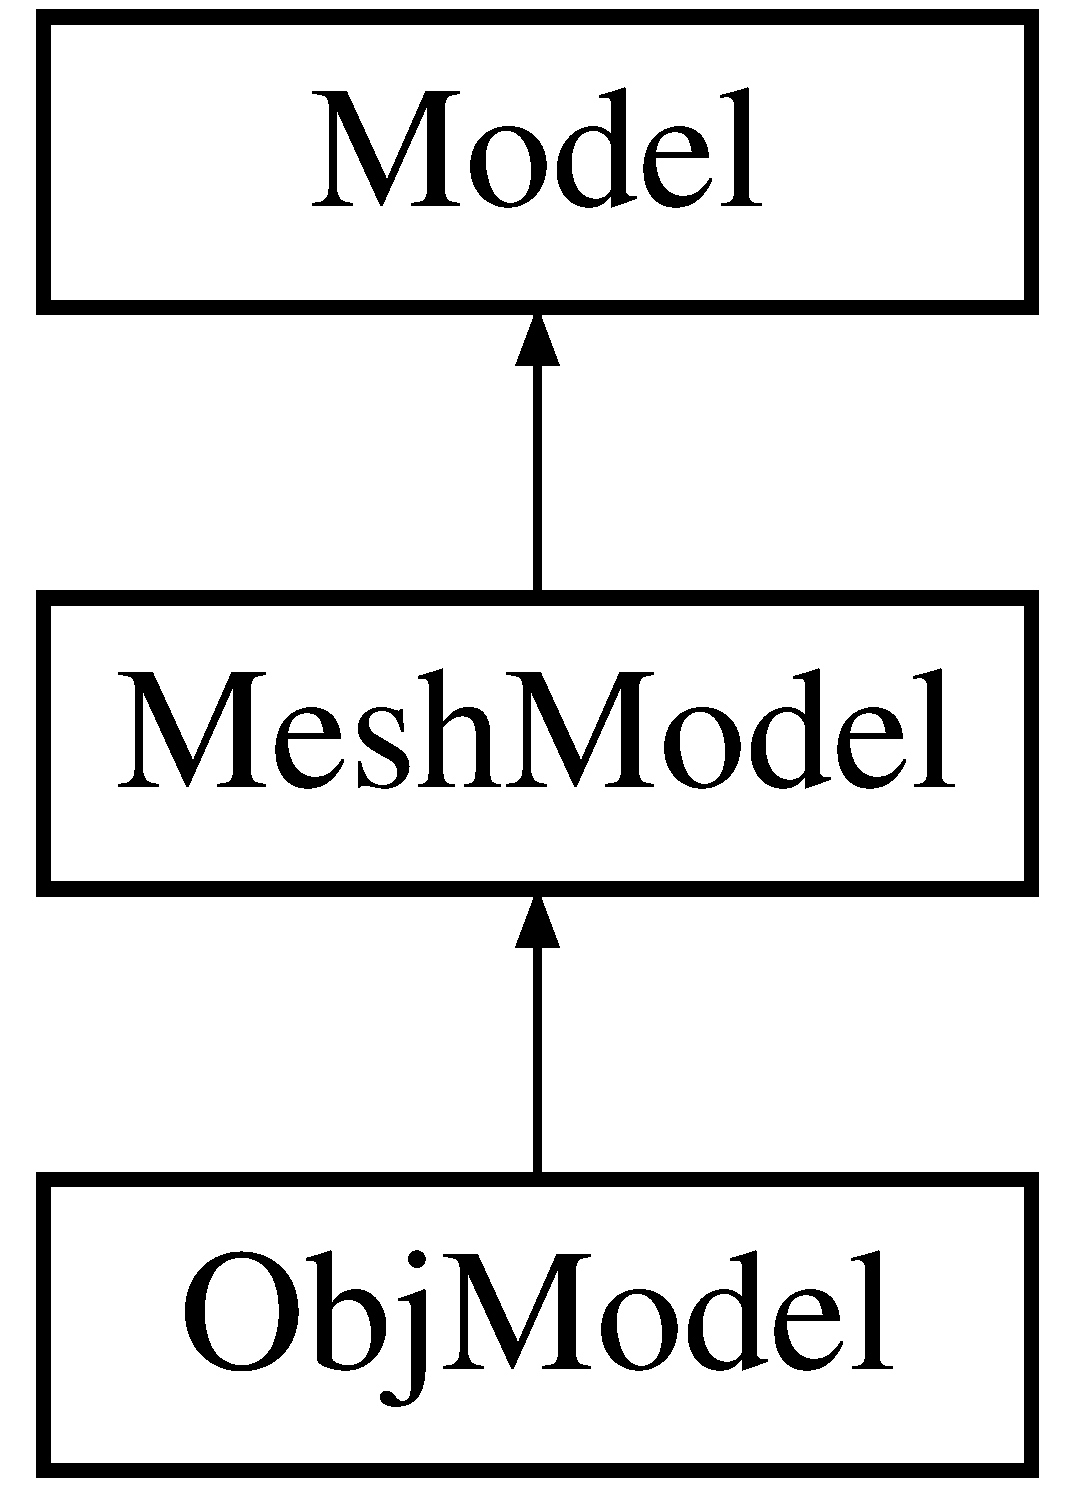
\includegraphics[height=3.000000cm]{classMeshModel}
\end{center}
\end{figure}
\subsection*{Public Member Functions}
\begin{DoxyCompactItemize}
\item 
\hypertarget{classMeshModel_a70765fc2bcc28904bdc0fd38eb8cd745}{\hyperlink{classMeshModel_a70765fc2bcc28904bdc0fd38eb8cd745}{Mesh\-Model} ()}\label{classMeshModel_a70765fc2bcc28904bdc0fd38eb8cd745}

\begin{DoxyCompactList}\small\item\em Default constructor does nothing but calling the \hyperlink{classModel_ae3b375de5f6df4faf74a95d64748e048}{Model()} constructor. \end{DoxyCompactList}\item 
\hypertarget{classMeshModel_acad5fe11036271fce2f7258f9cf3fbe4}{virtual \hyperlink{classMeshModel_acad5fe11036271fce2f7258f9cf3fbe4}{$\sim$\-Mesh\-Model} ()}\label{classMeshModel_acad5fe11036271fce2f7258f9cf3fbe4}

\begin{DoxyCompactList}\small\item\em Unimplemented destructor. \end{DoxyCompactList}\item 
\hypertarget{classMeshModel_a794db0d087fc1810cb3510ef0050ad28}{void \hyperlink{classMeshModel_a794db0d087fc1810cb3510ef0050ad28}{render} ()}\label{classMeshModel_a794db0d087fc1810cb3510ef0050ad28}

\begin{DoxyCompactList}\small\item\em Renders the \hyperlink{classMeshModel}{Mesh\-Model}. \end{DoxyCompactList}\item 
virtual void \hyperlink{classMeshModel_a79b1081f6b6ff72bf8fc24dc89578977}{read\-File} (char $\ast$filename)
\begin{DoxyCompactList}\small\item\em Reads \hyperlink{classMeshModel}{Mesh\-Model} data from a file. \end{DoxyCompactList}\end{DoxyCompactItemize}


\subsection{Member Function Documentation}
\hypertarget{classMeshModel_a79b1081f6b6ff72bf8fc24dc89578977}{\index{Mesh\-Model@{Mesh\-Model}!read\-File@{read\-File}}
\index{read\-File@{read\-File}!MeshModel@{Mesh\-Model}}
\subsubsection[{read\-File}]{\setlength{\rightskip}{0pt plus 5cm}void Mesh\-Model\-::read\-File (
\begin{DoxyParamCaption}
\item[{char $\ast$}]{filename}
\end{DoxyParamCaption}
)\hspace{0.3cm}{\ttfamily [virtual]}}}\label{classMeshModel_a79b1081f6b6ff72bf8fc24dc89578977}


Reads \hyperlink{classMeshModel}{Mesh\-Model} data from a file. 


\begin{DoxyParams}{Parameters}
{\em filename} & is the name of the data file. \\
\hline
\end{DoxyParams}


Reimplemented in \hyperlink{classObjModel_a99296bb22424ec9732ce3197991459d9}{Obj\-Model}.



The documentation for this class was generated from the following files\-:\begin{DoxyCompactItemize}
\item 
\hyperlink{meshmodel_8h}{meshmodel.\-h}\item 
meshmodel.\-cpp\end{DoxyCompactItemize}

\hypertarget{classModel}{\section{Model Class Reference}
\label{classModel}\index{Model@{Model}}
}
Inheritance diagram for Model\-:\begin{figure}[H]
\begin{center}
\leavevmode
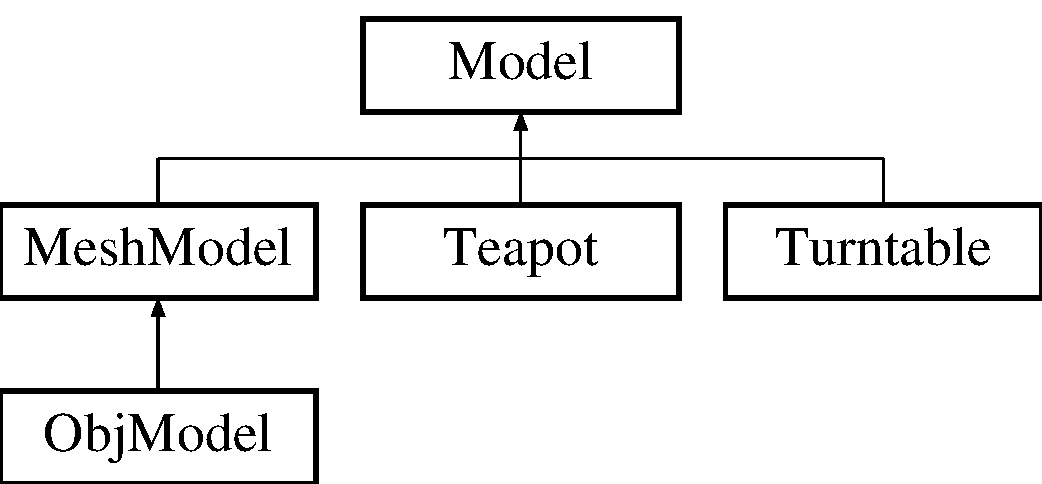
\includegraphics[height=3.000000cm]{classModel}
\end{center}
\end{figure}
\subsection*{Public Member Functions}
\begin{DoxyCompactItemize}
\item 
\hypertarget{classModel_ae3b375de5f6df4faf74a95d64748e048}{\hyperlink{classModel_ae3b375de5f6df4faf74a95d64748e048}{Model} ()}\label{classModel_ae3b375de5f6df4faf74a95d64748e048}

\begin{DoxyCompactList}\small\item\em Default constructor\-: only sets wireframe mode to false. \end{DoxyCompactList}\item 
\hypertarget{classModel_ad6ebd2062a0b823db841a0b88baac4c0}{virtual \hyperlink{classModel_ad6ebd2062a0b823db841a0b88baac4c0}{$\sim$\-Model} ()}\label{classModel_ad6ebd2062a0b823db841a0b88baac4c0}

\begin{DoxyCompactList}\small\item\em Unimplemented destructor. \end{DoxyCompactList}\item 
virtual void \hyperlink{classModel_a89ebd61864089abe5b0c5a1df6479970}{render} ()
\begin{DoxyCompactList}\small\item\em Placeholder for the render function. \end{DoxyCompactList}\item 
void \hyperlink{classModel_a9bbabfc8fba384132cac6a483bb31dd2}{set\-Wire\-Frame} (bool w)
\begin{DoxyCompactList}\small\item\em Setter function for wireframe/solid mode. \end{DoxyCompactList}\end{DoxyCompactItemize}


\subsection{Member Function Documentation}
\hypertarget{classModel_a89ebd61864089abe5b0c5a1df6479970}{\index{Model@{Model}!render@{render}}
\index{render@{render}!Model@{Model}}
\subsubsection[{render}]{\setlength{\rightskip}{0pt plus 5cm}void Model\-::render (
\begin{DoxyParamCaption}
{}
\end{DoxyParamCaption}
)\hspace{0.3cm}{\ttfamily [virtual]}}}\label{classModel_a89ebd61864089abe5b0c5a1df6479970}


Placeholder for the render function. 

Make sure you call this base (\hyperlink{classModel}{Model}) class' render function right at the start of your render function in the subclass. This one sets up the model so that the model can be viewed as both wireframe and solid. As we'll be placing the models on a turntable, one should ensure that the model is appropriately translated so that the lowest y-\/coordinate is set to zero. 

Reimplemented in \hyperlink{classObjModel_a490d057319a30734a0d6f27739f84565}{Obj\-Model}, \hyperlink{classTurntable_aaccddb594abd2665cf36fe5e2f6609cc}{Turntable}, \hyperlink{classTeapot_aababf7bd2833ebd3c34564b45b902163}{Teapot}, and \hyperlink{classMeshModel_a794db0d087fc1810cb3510ef0050ad28}{Mesh\-Model}.

\hypertarget{classModel_a9bbabfc8fba384132cac6a483bb31dd2}{\index{Model@{Model}!set\-Wire\-Frame@{set\-Wire\-Frame}}
\index{set\-Wire\-Frame@{set\-Wire\-Frame}!Model@{Model}}
\subsubsection[{set\-Wire\-Frame}]{\setlength{\rightskip}{0pt plus 5cm}void Model\-::set\-Wire\-Frame (
\begin{DoxyParamCaption}
\item[{bool}]{w}
\end{DoxyParamCaption}
)}}\label{classModel_a9bbabfc8fba384132cac6a483bb31dd2}


Setter function for wireframe/solid mode. 


\begin{DoxyParams}{Parameters}
{\em w} & is a boolean value indicating whether the model should be rendered as wireframe (true) or solid (false). \\
\hline
\end{DoxyParams}


The documentation for this class was generated from the following files\-:\begin{DoxyCompactItemize}
\item 
\hyperlink{model_8h}{model.\-h}\item 
model.\-cpp\end{DoxyCompactItemize}

\hypertarget{classNormal}{\section{Normal Class Reference}
\label{classNormal}\index{Normal@{Normal}}
}
\subsection*{Public Member Functions}
\begin{DoxyCompactItemize}
\item 
\hypertarget{classNormal_aea817fa6401166252c899d5e7a86dd0e}{{\bfseries Normal} (float i, float j, float k)}\label{classNormal_aea817fa6401166252c899d5e7a86dd0e}

\item 
\hypertarget{classNormal_a1616e612bec600893855682d971406b9}{void {\bfseries normalize} ()}\label{classNormal_a1616e612bec600893855682d971406b9}

\item 
\hypertarget{classNormal_a73aedd5b87467b934da29e54e653b309}{void {\bfseries use\-Normal} ()}\label{classNormal_a73aedd5b87467b934da29e54e653b309}

\end{DoxyCompactItemize}


The documentation for this class was generated from the following files\-:\begin{DoxyCompactItemize}
\item 
normal.\-h\item 
normal.\-cpp\end{DoxyCompactItemize}

\hypertarget{classObject}{\section{Object Class Reference}
\label{classObject}\index{Object@{Object}}
}
\subsection*{Public Member Functions}
\begin{DoxyCompactItemize}
\item 
\hypertarget{classObject_a536bd18bd32a3abae15cffd38e8f7861}{{\bfseries Object} (string name, \hyperlink{classObjModel}{Obj\-Model} $\ast$parent\-Model)}\label{classObject_a536bd18bd32a3abae15cffd38e8f7861}

\item 
\hypertarget{classObject_ae0e92359520b9a848f45efdd86485552}{void {\bfseries render} ()}\label{classObject_ae0e92359520b9a848f45efdd86485552}

\item 
\hypertarget{classObject_aea93aef61f2e464ccf297ea2be914e9a}{void {\bfseries add\-Face} (\hyperlink{classFace}{Face} face)}\label{classObject_aea93aef61f2e464ccf297ea2be914e9a}

\item 
\hypertarget{classObject_a9c5b41f17b960452065d2e6675655af0}{void {\bfseries print} ()}\label{classObject_a9c5b41f17b960452065d2e6675655af0}

\item 
\hypertarget{classObject_a5581cddd8e15ff480cc60f0e2715eecb}{bool {\bfseries is\-Null} ()}\label{classObject_a5581cddd8e15ff480cc60f0e2715eecb}

\end{DoxyCompactItemize}


The documentation for this class was generated from the following files\-:\begin{DoxyCompactItemize}
\item 
object.\-h\item 
object.\-cpp\end{DoxyCompactItemize}

\hypertarget{classObjModel}{\section{Obj\-Model Class Reference}
\label{classObjModel}\index{Obj\-Model@{Obj\-Model}}
}
Inheritance diagram for Obj\-Model\-:\begin{figure}[H]
\begin{center}
\leavevmode
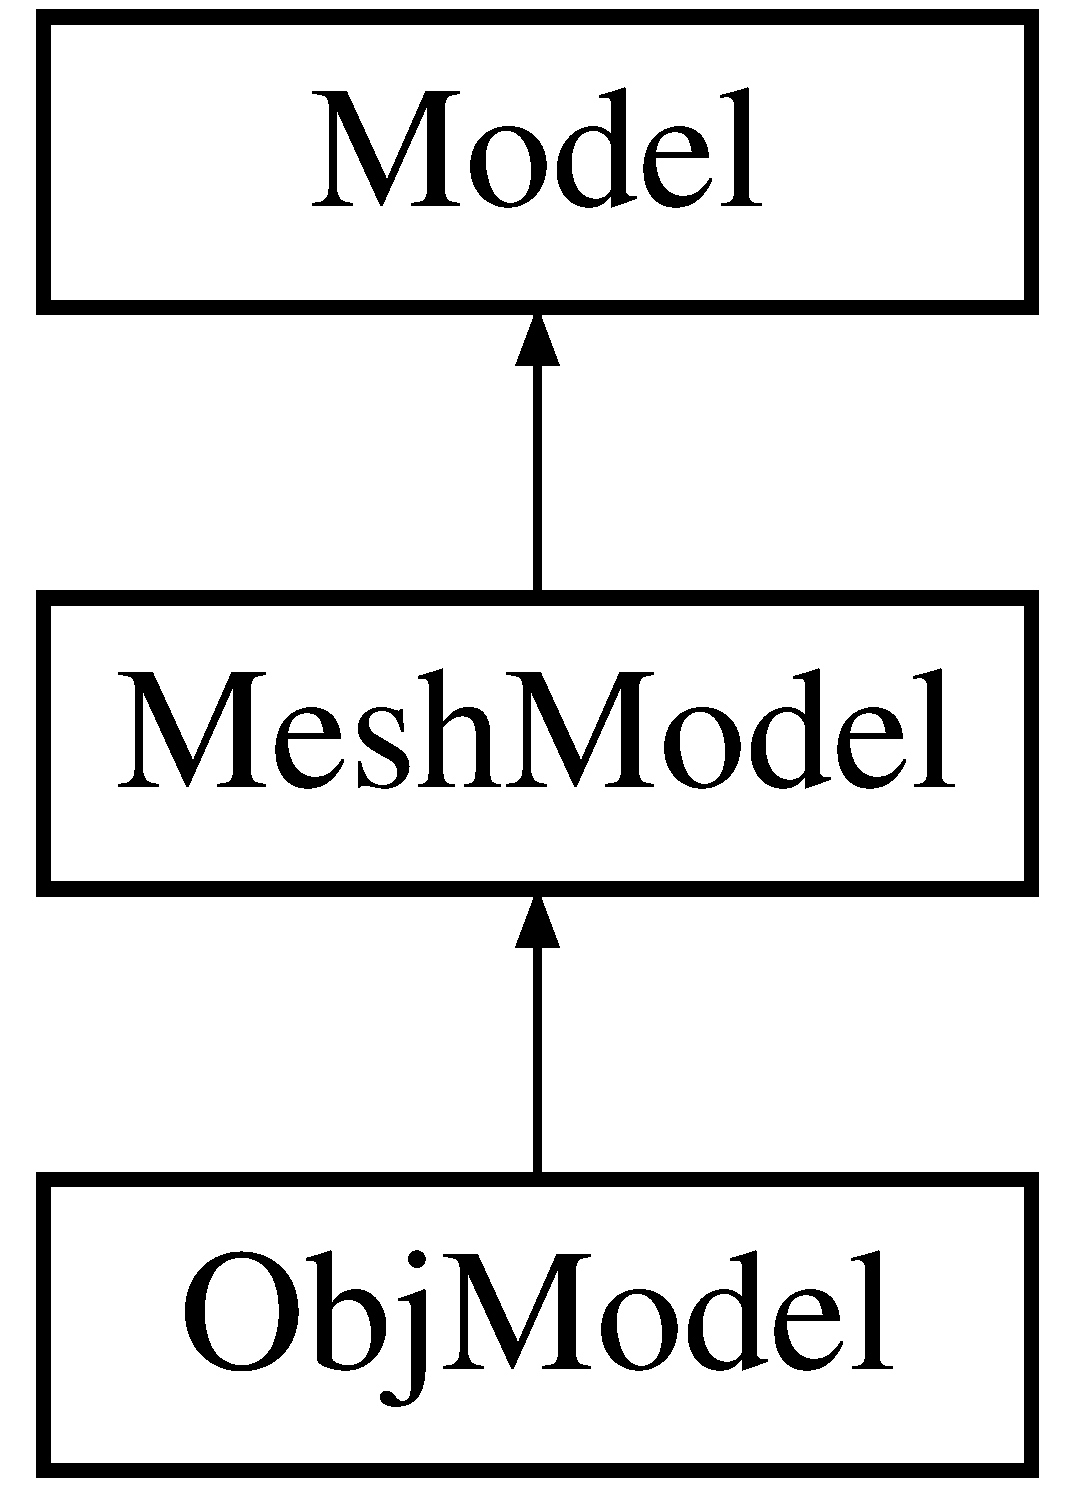
\includegraphics[height=3.000000cm]{classObjModel}
\end{center}
\end{figure}
\subsection*{Public Member Functions}
\begin{DoxyCompactItemize}
\item 
\hypertarget{classObjModel_af7c00f757992e626f2dd959f4c829125}{\hyperlink{classObjModel_af7c00f757992e626f2dd959f4c829125}{Obj\-Model} ()}\label{classObjModel_af7c00f757992e626f2dd959f4c829125}

\begin{DoxyCompactList}\small\item\em Default constructor does nothing but calling the \hyperlink{classModel_ae3b375de5f6df4faf74a95d64748e048}{Model()} constructor. \end{DoxyCompactList}\item 
\hypertarget{classObjModel_a78d50e0da345b8b2438bbc93ae01eab8}{virtual \hyperlink{classObjModel_a78d50e0da345b8b2438bbc93ae01eab8}{$\sim$\-Obj\-Model} ()}\label{classObjModel_a78d50e0da345b8b2438bbc93ae01eab8}

\begin{DoxyCompactList}\small\item\em Unimplemented destructor. \end{DoxyCompactList}\item 
void \hyperlink{classObjModel_a490d057319a30734a0d6f27739f84565}{render} ()
\begin{DoxyCompactList}\small\item\em Renders the \hyperlink{classObjModel}{Obj\-Model}. \end{DoxyCompactList}\item 
virtual void \hyperlink{classObjModel_a99296bb22424ec9732ce3197991459d9}{read\-File} (char $\ast$filename)
\begin{DoxyCompactList}\small\item\em Reads \hyperlink{classObjModel}{Obj\-Model} mesh data from a .obj file and material data from .mtl file. \end{DoxyCompactList}\item 
\hypertarget{classObjModel_ad5cf8b20897f7d745ef5cf5121e1e3e2}{bool \hyperlink{classObjModel_ad5cf8b20897f7d745ef5cf5121e1e3e2}{is\-Ready} ()}\label{classObjModel_ad5cf8b20897f7d745ef5cf5121e1e3e2}

\begin{DoxyCompactList}\small\item\em Returns true if the model is ready to be rendered, false otherwise. \end{DoxyCompactList}\item 
\hypertarget{classObjModel_a2cd661ed082445bbee4bca792042693c}{vector$<$ \hyperlink{classVertex}{Vertex} $>$ $\ast$ {\bfseries get\-Vertices} ()}\label{classObjModel_a2cd661ed082445bbee4bca792042693c}

\end{DoxyCompactItemize}


\subsection{Member Function Documentation}
\hypertarget{classObjModel_a99296bb22424ec9732ce3197991459d9}{\index{Obj\-Model@{Obj\-Model}!read\-File@{read\-File}}
\index{read\-File@{read\-File}!ObjModel@{Obj\-Model}}
\subsubsection[{read\-File}]{\setlength{\rightskip}{0pt plus 5cm}void Obj\-Model\-::read\-File (
\begin{DoxyParamCaption}
\item[{char $\ast$}]{filename}
\end{DoxyParamCaption}
)\hspace{0.3cm}{\ttfamily [virtual]}}}\label{classObjModel_a99296bb22424ec9732ce3197991459d9}


Reads \hyperlink{classObjModel}{Obj\-Model} mesh data from a .obj file and material data from .mtl file. 


\begin{DoxyParams}{Parameters}
{\em filename} & is the base name (without extension) of the data files (for example\-: teapot, not teapot.\-obj).\\
\hline
\end{DoxyParams}
You need to implement this function properly.

\begin{DoxyWarning}{Warning}
you need to uncomment a line in this function to let \hyperlink{main_8cpp}{main.\-cpp} know that we're ready to render. 
\end{DoxyWarning}


Reimplemented from \hyperlink{classMeshModel_a79b1081f6b6ff72bf8fc24dc89578977}{Mesh\-Model}.

\hypertarget{classObjModel_a490d057319a30734a0d6f27739f84565}{\index{Obj\-Model@{Obj\-Model}!render@{render}}
\index{render@{render}!ObjModel@{Obj\-Model}}
\subsubsection[{render}]{\setlength{\rightskip}{0pt plus 5cm}void Obj\-Model\-::render (
\begin{DoxyParamCaption}
{}
\end{DoxyParamCaption}
)\hspace{0.3cm}{\ttfamily [virtual]}}}\label{classObjModel_a490d057319a30734a0d6f27739f84565}


Renders the \hyperlink{classObjModel}{Obj\-Model}. 

You need to implement this function properly. Make sure you translate your model so that it stands on the zx-\/plane. The lowest y-\/coordinate needs to be at zero. 

Reimplemented from \hyperlink{classMeshModel_a794db0d087fc1810cb3510ef0050ad28}{Mesh\-Model}.



The documentation for this class was generated from the following files\-:\begin{DoxyCompactItemize}
\item 
\hyperlink{objmodel_8h}{objmodel.\-h}\item 
objmodel.\-cpp\end{DoxyCompactItemize}

\hypertarget{classTeapot}{\section{Teapot Class Reference}
\label{classTeapot}\index{Teapot@{Teapot}}
}
Inheritance diagram for Teapot\-:\begin{figure}[H]
\begin{center}
\leavevmode
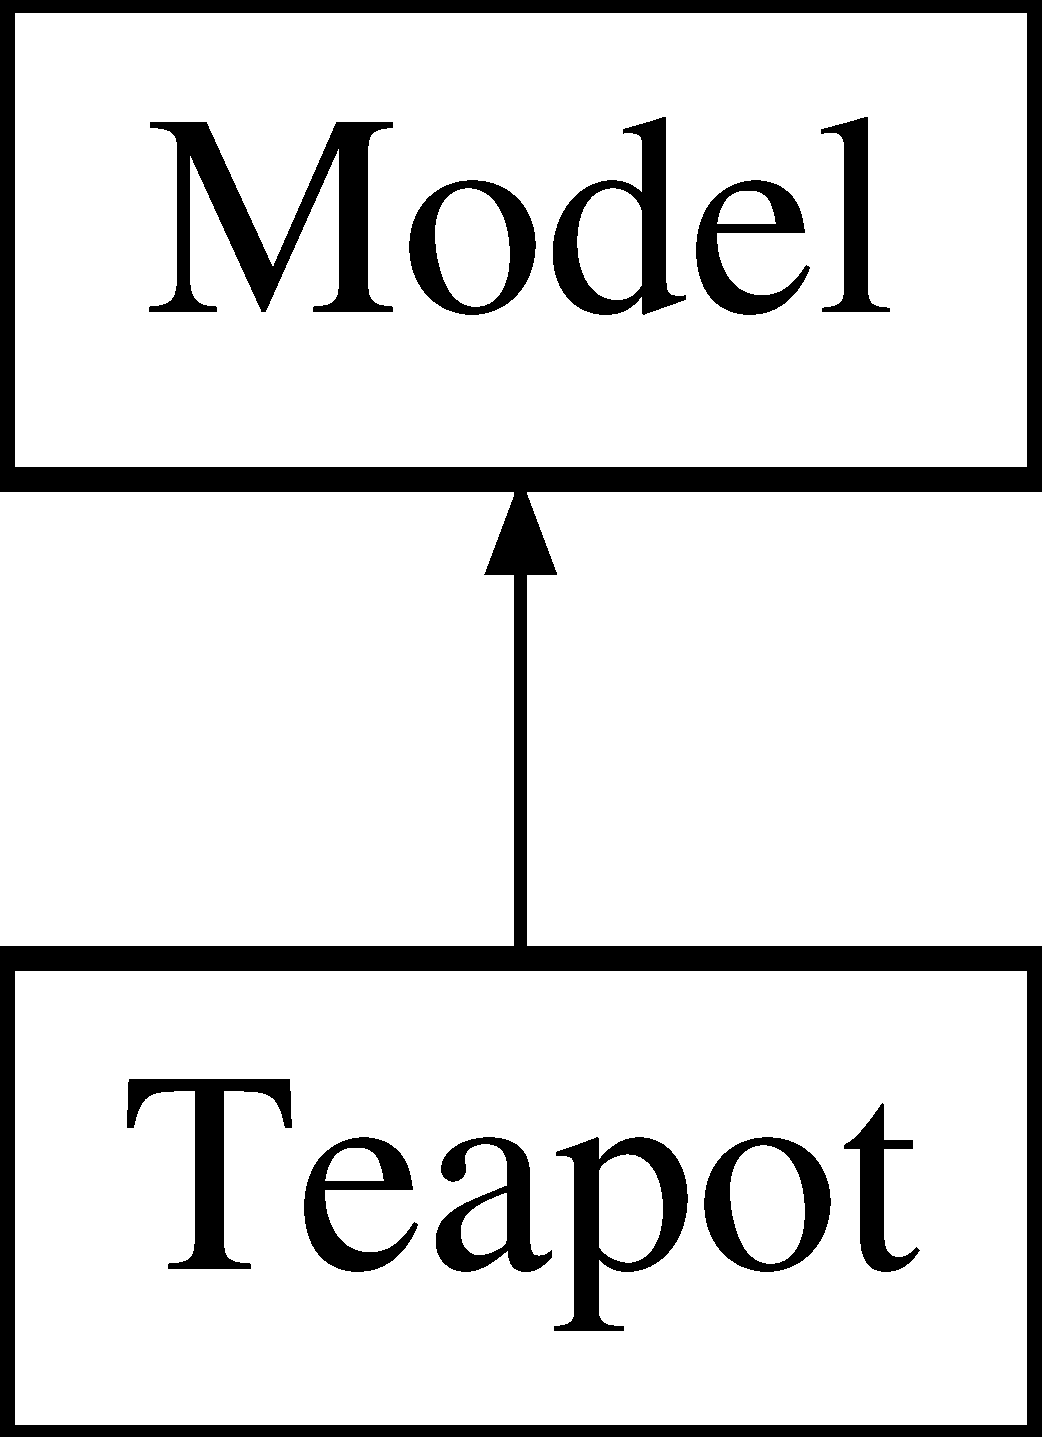
\includegraphics[height=2.000000cm]{classTeapot}
\end{center}
\end{figure}
\subsection*{Public Member Functions}
\begin{DoxyCompactItemize}
\item 
\hypertarget{classTeapot_aeb69723c977accc5a84cf958e492accd}{\hyperlink{classTeapot_aeb69723c977accc5a84cf958e492accd}{Teapot} ()}\label{classTeapot_aeb69723c977accc5a84cf958e492accd}

\begin{DoxyCompactList}\small\item\em Default constructor does nothing but calling the \hyperlink{classModel_ae3b375de5f6df4faf74a95d64748e048}{Model()} constructor. \end{DoxyCompactList}\item 
\hyperlink{classTeapot_ad64f28b4c9da6dba20f93b949af2522f}{Teapot} (double s)
\begin{DoxyCompactList}\small\item\em Overloaded constructor that takes size of the teapot as input. \end{DoxyCompactList}\item 
\hypertarget{classTeapot_a1c243d488157da74b0e1a2412a921f00}{\hyperlink{classTeapot_a1c243d488157da74b0e1a2412a921f00}{$\sim$\-Teapot} ()}\label{classTeapot_a1c243d488157da74b0e1a2412a921f00}

\begin{DoxyCompactList}\small\item\em Unimplemented destructor. Doesn't have anything to free up. \end{DoxyCompactList}\item 
\hypertarget{classTeapot_aababf7bd2833ebd3c34564b45b902163}{void \hyperlink{classTeapot_aababf7bd2833ebd3c34564b45b902163}{render} ()}\label{classTeapot_aababf7bd2833ebd3c34564b45b902163}

\begin{DoxyCompactList}\small\item\em Renders the teapot. \end{DoxyCompactList}\end{DoxyCompactItemize}


\subsection{Constructor \& Destructor Documentation}
\hypertarget{classTeapot_ad64f28b4c9da6dba20f93b949af2522f}{\index{Teapot@{Teapot}!Teapot@{Teapot}}
\index{Teapot@{Teapot}!Teapot@{Teapot}}
\subsubsection[{Teapot}]{\setlength{\rightskip}{0pt plus 5cm}Teapot\-::\-Teapot (
\begin{DoxyParamCaption}
\item[{double}]{s}
\end{DoxyParamCaption}
)}}\label{classTeapot_ad64f28b4c9da6dba20f93b949af2522f}


Overloaded constructor that takes size of the teapot as input. 


\begin{DoxyParams}{Parameters}
{\em s} & is the relative size of the teapot. \\
\hline
\end{DoxyParams}


The documentation for this class was generated from the following files\-:\begin{DoxyCompactItemize}
\item 
\hyperlink{teapot_8h}{teapot.\-h}\item 
teapot.\-cpp\end{DoxyCompactItemize}

\hypertarget{classTurntable}{\section{Turntable Class Reference}
\label{classTurntable}\index{Turntable@{Turntable}}
}
Inheritance diagram for Turntable\-:\begin{figure}[H]
\begin{center}
\leavevmode
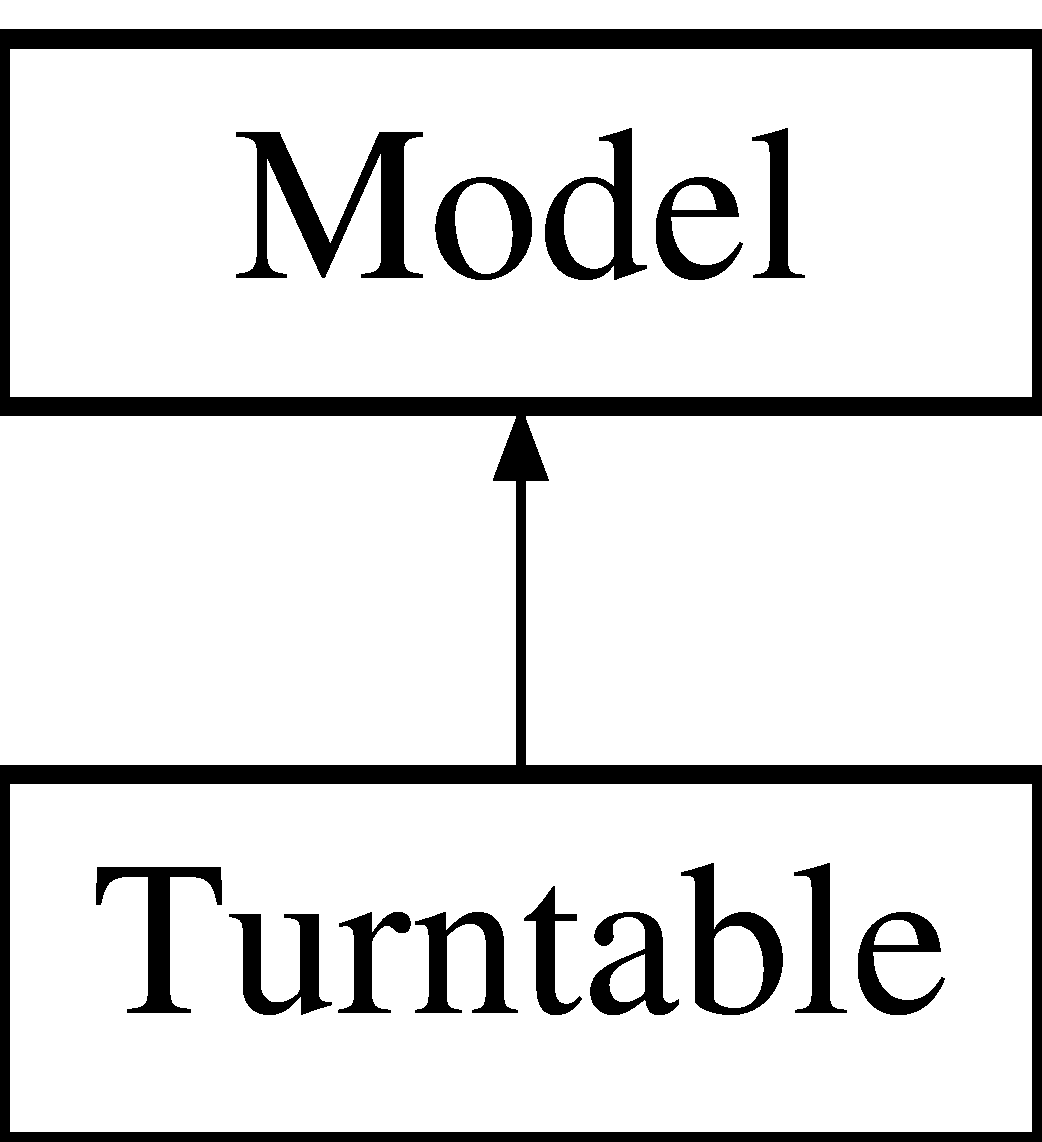
\includegraphics[height=2.000000cm]{classTurntable}
\end{center}
\end{figure}
\subsection*{Public Member Functions}
\begin{DoxyCompactItemize}
\item 
\hyperlink{classTurntable_a630b239cf4edd80dd1f2b9e006afb824}{Turntable} ()
\begin{DoxyCompactList}\small\item\em Default constructor for the \hyperlink{classTurntable}{Turntable} class. \end{DoxyCompactList}\item 
\hyperlink{classTurntable_a3a73c1ca03efd0d05f2b3903923bdb89}{Turntable} (double r, double h)
\begin{DoxyCompactList}\small\item\em Overloaded constructor that takes radius and height as parameters. \end{DoxyCompactList}\item 
void \hyperlink{classTurntable_aaccddb594abd2665cf36fe5e2f6609cc}{render} ()
\begin{DoxyCompactList}\small\item\em Renders the turntable flat out on the zx-\/plane. \end{DoxyCompactList}\end{DoxyCompactItemize}


\subsection{Constructor \& Destructor Documentation}
\hypertarget{classTurntable_a630b239cf4edd80dd1f2b9e006afb824}{\index{Turntable@{Turntable}!Turntable@{Turntable}}
\index{Turntable@{Turntable}!Turntable@{Turntable}}
\subsubsection[{Turntable}]{\setlength{\rightskip}{0pt plus 5cm}Turntable\-::\-Turntable (
\begin{DoxyParamCaption}
{}
\end{DoxyParamCaption}
)}}\label{classTurntable_a630b239cf4edd80dd1f2b9e006afb824}


Default constructor for the \hyperlink{classTurntable}{Turntable} class. 

Simply calls the \hyperlink{classModel_ae3b375de5f6df4faf74a95d64748e048}{Model()} constructor of the base class \hyperlink{classModel}{Model}. \hypertarget{classTurntable_a3a73c1ca03efd0d05f2b3903923bdb89}{\index{Turntable@{Turntable}!Turntable@{Turntable}}
\index{Turntable@{Turntable}!Turntable@{Turntable}}
\subsubsection[{Turntable}]{\setlength{\rightskip}{0pt plus 5cm}Turntable\-::\-Turntable (
\begin{DoxyParamCaption}
\item[{double}]{r, }
\item[{double}]{h}
\end{DoxyParamCaption}
)}}\label{classTurntable_a3a73c1ca03efd0d05f2b3903923bdb89}


Overloaded constructor that takes radius and height as parameters. 

Calls the default constructor \hyperlink{classTurntable_a630b239cf4edd80dd1f2b9e006afb824}{Turntable()} first and then sets up radius and height as passed. 
\begin{DoxyParams}{Parameters}
{\em r} & is the radius \\
\hline
{\em h} & is the height \\
\hline
\end{DoxyParams}


\subsection{Member Function Documentation}
\hypertarget{classTurntable_aaccddb594abd2665cf36fe5e2f6609cc}{\index{Turntable@{Turntable}!render@{render}}
\index{render@{render}!Turntable@{Turntable}}
\subsubsection[{render}]{\setlength{\rightskip}{0pt plus 5cm}void Turntable\-::render (
\begin{DoxyParamCaption}
{}
\end{DoxyParamCaption}
)\hspace{0.3cm}{\ttfamily [virtual]}}}\label{classTurntable_aaccddb594abd2665cf36fe5e2f6609cc}


Renders the turntable flat out on the zx-\/plane. 

The turntable is created with 3 tapered cylinders using glu\-Cylinder() function calls. The topmost cylinder has top radius set to zero giving an appearance of closed off lid to the base cylinder. 

Reimplemented from \hyperlink{classModel_a89ebd61864089abe5b0c5a1df6479970}{Model}.



The documentation for this class was generated from the following files\-:\begin{DoxyCompactItemize}
\item 
\hyperlink{turntable_8h}{turntable.\-h}\item 
turntable.\-cpp\end{DoxyCompactItemize}

\hypertarget{classVertex}{\section{Vertex Class Reference}
\label{classVertex}\index{Vertex@{Vertex}}
}
\subsection*{Public Member Functions}
\begin{DoxyCompactItemize}
\item 
\hypertarget{classVertex_a2c558c054a0a2c970588c063073803a0}{{\bfseries Vertex} (float x, float y, float z)}\label{classVertex_a2c558c054a0a2c970588c063073803a0}

\item 
\hypertarget{classVertex_aa78d4c3433559e6e50260240c49a3d03}{float {\bfseries get\-X} ()}\label{classVertex_aa78d4c3433559e6e50260240c49a3d03}

\item 
\hypertarget{classVertex_a12facdc9f554fd718e449f2aa2eefeaf}{float {\bfseries get\-Y} ()}\label{classVertex_a12facdc9f554fd718e449f2aa2eefeaf}

\item 
\hypertarget{classVertex_a258fea59f7c07f4e8784fc90c6ac7cb3}{float {\bfseries get\-Z} ()}\label{classVertex_a258fea59f7c07f4e8784fc90c6ac7cb3}

\end{DoxyCompactItemize}


The documentation for this class was generated from the following files\-:\begin{DoxyCompactItemize}
\item 
vertex.\-h\item 
vertex.\-cpp\end{DoxyCompactItemize}

\chapter{File Documentation}
\hypertarget{light_8h}{\section{light.\-h File Reference}
\label{light_8h}\index{light.\-h@{light.\-h}}
}


A simple \hyperlink{classLight}{Light} class to facilitate light control in the scene.  


{\ttfamily \#include $<$G\-L/glut.\-h$>$}\\*
\subsection*{Classes}
\begin{DoxyCompactItemize}
\item 
class \hyperlink{classLight}{Light}
\end{DoxyCompactItemize}


\subsection{Detailed Description}
A simple \hyperlink{classLight}{Light} class to facilitate light control in the scene. \begin{DoxyAuthor}{Author}
Monirul Hasan \href{mailto:kmhasan@gmail.com}{\tt kmhasan@gmail.\-com} 
\end{DoxyAuthor}
\begin{DoxyDate}{Date}
March 2014 
\end{DoxyDate}

\hypertarget{main_8cpp}{\section{main.\-cpp File Reference}
\label{main_8cpp}\index{main.\-cpp@{main.\-cpp}}
}


Summer 2015 Assignment \#2.  


{\ttfamily \#include $<$G\-L/glut.\-h$>$}\\*
{\ttfamily \#include $<$cmath$>$}\\*
{\ttfamily \#include $<$chrono$>$}\\*
{\ttfamily \#include $<$iostream$>$}\\*
{\ttfamily \#include $<$string$>$}\\*
{\ttfamily \#include $<$pthread.\-h$>$}\\*
{\ttfamily \#include \char`\"{}model.\-h\char`\"{}}\\*
{\ttfamily \#include \char`\"{}teapot.\-h\char`\"{}}\\*
{\ttfamily \#include \char`\"{}turntable.\-h\char`\"{}}\\*
{\ttfamily \#include \char`\"{}light.\-h\char`\"{}}\\*
{\ttfamily \#include \char`\"{}meshmodel.\-h\char`\"{}}\\*
{\ttfamily \#include \char`\"{}objmodel.\-h\char`\"{}}\\*
\subsection*{Functions}
\begin{DoxyCompactItemize}
\item 
void \hyperlink{main_8cpp_ab5faa224cc65d6fbce2935d0ed45f600}{draw\-Grid} ()
\begin{DoxyCompactList}\small\item\em Draws a 2\-D grid on zx-\/plane. \end{DoxyCompactList}\item 
void \hyperlink{main_8cpp_ab3131ecac9dbbafaf695e4c14588cbe6}{spin\-Me} ()
\begin{DoxyCompactList}\small\item\em Spins the \hyperlink{classTurntable}{Turntable} along with the \hyperlink{classModel}{Model} on top of it about the y-\/axis. \end{DoxyCompactList}\item 
void \hyperlink{main_8cpp_a02fd73d861ef2e4aabb38c0c9ff82947}{init} ()
\begin{DoxyCompactList}\small\item\em Initialization function to instantiate objects and to do related tasks. \end{DoxyCompactList}\item 
\hypertarget{main_8cpp_a1e5b20fed15743656bb6d2e6a6ea6269}{void \hyperlink{main_8cpp_a1e5b20fed15743656bb6d2e6a6ea6269}{display} ()}\label{main_8cpp_a1e5b20fed15743656bb6d2e6a6ea6269}

\begin{DoxyCompactList}\small\item\em The \hyperlink{main_8cpp_a1e5b20fed15743656bb6d2e6a6ea6269}{display()} callback function. \end{DoxyCompactList}\item 
void \hyperlink{main_8cpp_a6819355374dd277347abd7c4235f0cd7}{reshape} (int width, int height)
\begin{DoxyCompactList}\small\item\em The \hyperlink{main_8cpp_a6819355374dd277347abd7c4235f0cd7}{reshape()} callback function. \end{DoxyCompactList}\item 
void \hyperlink{main_8cpp_a11bf38c6c77e542db015911b24bedc30}{keyboard} (unsigned char ch, int x, int y)
\begin{DoxyCompactList}\small\item\em The \hyperlink{main_8cpp_a11bf38c6c77e542db015911b24bedc30}{keyboard()} callback function. \end{DoxyCompactList}\item 
int \hyperlink{main_8cpp_a3c04138a5bfe5d72780bb7e82a18e627}{main} (int argc, char $\ast$$\ast$argv)
\begin{DoxyCompactList}\small\item\em The main function to start it all! \end{DoxyCompactList}\end{DoxyCompactItemize}
\subsection*{Variables}
\begin{DoxyCompactItemize}
\item 
\hypertarget{main_8cpp_a1b4ff01fffb1ae04ef35d0c777ff86ea}{chrono\-::time\-\_\-point\\*
$<$ chrono\-::system\-\_\-clock $>$ \hyperlink{main_8cpp_a1b4ff01fffb1ae04ef35d0c777ff86ea}{last}}\label{main_8cpp_a1b4ff01fffb1ae04ef35d0c777ff86ea}

\begin{DoxyCompactList}\small\item\em C++11 extension chrono classes to track time spent in between frames -- last time\-\_\-point. \end{DoxyCompactList}\item 
\hypertarget{main_8cpp_ab534d9990d3a1fca6ba8d20301781429}{chrono\-::time\-\_\-point\\*
$<$ chrono\-::system\-\_\-clock $>$ \hyperlink{main_8cpp_ab534d9990d3a1fca6ba8d20301781429}{current}}\label{main_8cpp_ab534d9990d3a1fca6ba8d20301781429}

\begin{DoxyCompactList}\small\item\em C++11 extension chrono classes to track time spent in between frames -- current time\-\_\-point. \end{DoxyCompactList}\item 
\hypertarget{main_8cpp_ad06bc4182f3264c41aa3d010eb4b03ee}{const double \hyperlink{main_8cpp_ad06bc4182f3264c41aa3d010eb4b03ee}{turntable\-Height} = 0.\-5}\label{main_8cpp_ad06bc4182f3264c41aa3d010eb4b03ee}

\begin{DoxyCompactList}\small\item\em base height of the \hyperlink{classTurntable}{Turntable} -- used to translate the model so that it sits on zx-\/plane \end{DoxyCompactList}\item 
\hypertarget{main_8cpp_a55c5348c81be8a6efb487d0f8d6374c4}{const double \hyperlink{main_8cpp_a55c5348c81be8a6efb487d0f8d6374c4}{turntable\-Radius} = 7.\-0}\label{main_8cpp_a55c5348c81be8a6efb487d0f8d6374c4}

\begin{DoxyCompactList}\small\item\em base radius of the \hyperlink{classTurntable}{Turntable} \end{DoxyCompactList}\item 
\hypertarget{main_8cpp_a87accd1af8e0aff4b818d891374f7cec}{double \hyperlink{main_8cpp_a87accd1af8e0aff4b818d891374f7cec}{t} = 0}\label{main_8cpp_a87accd1af8e0aff4b818d891374f7cec}

\begin{DoxyCompactList}\small\item\em time t in seconds \end{DoxyCompactList}\item 
\hypertarget{main_8cpp_a62ab25ca0dac52cd5b575b88acbf69be}{float \hyperlink{main_8cpp_a62ab25ca0dac52cd5b575b88acbf69be}{spin} = 0.\-0}\label{main_8cpp_a62ab25ca0dac52cd5b575b88acbf69be}

\begin{DoxyCompactList}\small\item\em the spin angle to control the rotation of turntable about the y-\/axis \end{DoxyCompactList}\item 
\hypertarget{main_8cpp_a11926af9280d70fd96e47b07c90cf0ed}{double \hyperlink{main_8cpp_a11926af9280d70fd96e47b07c90cf0ed}{aspect} = 1.\-0}\label{main_8cpp_a11926af9280d70fd96e47b07c90cf0ed}

\begin{DoxyCompactList}\small\item\em aspect ratio (width\-:height) of the window \end{DoxyCompactList}\item 
\hypertarget{main_8cpp_a66076fd4c94f1ef66bb0256b653cf37f}{bool \hyperlink{main_8cpp_a66076fd4c94f1ef66bb0256b653cf37f}{pause} = false}\label{main_8cpp_a66076fd4c94f1ef66bb0256b653cf37f}

\begin{DoxyCompactList}\small\item\em flag to toggle turntable rotation on or off \end{DoxyCompactList}\item 
\hypertarget{main_8cpp_a08a3667327ce020588b5451aa2c2fb8e}{char \hyperlink{main_8cpp_a08a3667327ce020588b5451aa2c2fb8e}{axis\-Selection} = '\textbackslash{}0'}\label{main_8cpp_a08a3667327ce020588b5451aa2c2fb8e}

\begin{DoxyCompactList}\small\item\em marks which axis is selected for camera movement \end{DoxyCompactList}\item 
\hypertarget{main_8cpp_aa53f6b8a238b0ee4ffbfda54d8c713a3}{char \hyperlink{main_8cpp_aa53f6b8a238b0ee4ffbfda54d8c713a3}{light\-Selection} = '\textbackslash{}0'}\label{main_8cpp_aa53f6b8a238b0ee4ffbfda54d8c713a3}

\begin{DoxyCompactList}\small\item\em marks which light is selected to be turned on or off \end{DoxyCompactList}\item 
\hypertarget{main_8cpp_a9fe883a18727d129289b149e5f0305eb}{double \hyperlink{main_8cpp_a9fe883a18727d129289b149e5f0305eb}{cam} \mbox{[}3\mbox{]} = \{18, 6, 18\}}\label{main_8cpp_a9fe883a18727d129289b149e5f0305eb}

\begin{DoxyCompactList}\small\item\em initial location of the camera \end{DoxyCompactList}\item 
\hypertarget{main_8cpp_a8a386eee5b2436261bfa1fc0f4bcfa6e}{\hyperlink{classModel}{Model} $\ast$ \hyperlink{main_8cpp_a8a386eee5b2436261bfa1fc0f4bcfa6e}{turntable}}\label{main_8cpp_a8a386eee5b2436261bfa1fc0f4bcfa6e}

\begin{DoxyCompactList}\small\item\em pointer to the \hyperlink{classTurntable}{Turntable} \end{DoxyCompactList}\item 
\hypertarget{main_8cpp_a7b56c3ca57dde73bdbc8dbe9772bca19}{\hyperlink{classModel}{Model} $\ast$ \hyperlink{main_8cpp_a7b56c3ca57dde73bdbc8dbe9772bca19}{model}}\label{main_8cpp_a7b56c3ca57dde73bdbc8dbe9772bca19}

\begin{DoxyCompactList}\small\item\em pointer to the \hyperlink{classModel}{Model} to be placed on the \hyperlink{classTurntable}{Turntable} \end{DoxyCompactList}\item 
\hypertarget{main_8cpp_a5743fe18cdbdb6f65e0aa1635b52f8db}{\hyperlink{classLight}{Light} $\ast$ \hyperlink{main_8cpp_a5743fe18cdbdb6f65e0aa1635b52f8db}{light} \mbox{[}3\mbox{]}}\label{main_8cpp_a5743fe18cdbdb6f65e0aa1635b52f8db}

\begin{DoxyCompactList}\small\item\em pointers to the \hyperlink{classLight}{Light} (s) in the scene \end{DoxyCompactList}\item 
\hypertarget{main_8cpp_a746d3380ab43f61760f426f4d572331f}{\hyperlink{classModel}{Model} $\ast$ {\bfseries another\-Model}}\label{main_8cpp_a746d3380ab43f61760f426f4d572331f}

\end{DoxyCompactItemize}


\subsection{Detailed Description}
Summer 2015 Assignment \#2. \begin{DoxyAuthor}{Author}
Monirul Hasan \href{mailto:kmhasan@gmail.com}{\tt kmhasan@gmail.\-com} 
\end{DoxyAuthor}
\begin{DoxyDate}{Date}
July 7, 2015
\end{DoxyDate}
Submission deadline\-: 11\-:59 P\-M Friday July 24, 2014

Email subject line\-: C\-S\-E4013\-Spring2014\-A3

Task\-: Load a car model (preferably the one you submitted for the previous assignment) and drive it. As it is, the model loads up just fine, but the faces render flat shaded. You need to export the obj with the vertex normals written out in the .obj file. You also need to modify the file reading code so that it can handle vertex normal information. Figure out how you can set normals in Open\-G\-L and how to get Open\-G\-L to show the model smooth shaded. As for driving the car, at the very least you need to have the wheels rotate and the car move forward.

\begin{DoxyWarning}{Warning}
Any sign of copying will result in a zero score for everyone involved. Depending on the severity of the offense, I may issue further penalty. 
\end{DoxyWarning}


\subsection{Function Documentation}
\hypertarget{main_8cpp_ab5faa224cc65d6fbce2935d0ed45f600}{\index{main.\-cpp@{main.\-cpp}!draw\-Grid@{draw\-Grid}}
\index{draw\-Grid@{draw\-Grid}!main.cpp@{main.\-cpp}}
\subsubsection[{draw\-Grid}]{\setlength{\rightskip}{0pt plus 5cm}void draw\-Grid (
\begin{DoxyParamCaption}
{}
\end{DoxyParamCaption}
)}}\label{main_8cpp_ab5faa224cc65d6fbce2935d0ed45f600}


Draws a 2\-D grid on zx-\/plane. 

Dimension of the grid drawn is 20 x 20. \hypertarget{main_8cpp_a02fd73d861ef2e4aabb38c0c9ff82947}{\index{main.\-cpp@{main.\-cpp}!init@{init}}
\index{init@{init}!main.cpp@{main.\-cpp}}
\subsubsection[{init}]{\setlength{\rightskip}{0pt plus 5cm}void init (
\begin{DoxyParamCaption}
{}
\end{DoxyParamCaption}
)}}\label{main_8cpp_a02fd73d861ef2e4aabb38c0c9ff82947}


Initialization function to instantiate objects and to do related tasks. 

Instantiates a \hyperlink{classTurntable}{Turntable}, a \hyperlink{classTeapot}{Teapot} for a model, two lights and sets backface culling on. \hypertarget{main_8cpp_a11bf38c6c77e542db015911b24bedc30}{\index{main.\-cpp@{main.\-cpp}!keyboard@{keyboard}}
\index{keyboard@{keyboard}!main.cpp@{main.\-cpp}}
\subsubsection[{keyboard}]{\setlength{\rightskip}{0pt plus 5cm}void keyboard (
\begin{DoxyParamCaption}
\item[{unsigned char}]{ch, }
\item[{int}]{x, }
\item[{int}]{y}
\end{DoxyParamCaption}
)}}\label{main_8cpp_a11bf38c6c77e542db015911b24bedc30}


The \hyperlink{main_8cpp_a11bf38c6c77e542db015911b24bedc30}{keyboard()} callback function. 


\begin{DoxyParams}{Parameters}
{\em ch} & is the character that's pressed. \\
\hline
{\em x} & is the x-\/coordinate of the mouse when key is pressed \\
\hline
{\em y} & is the y-\/coordinate of the mouse when key is pressed\\
\hline
\end{DoxyParams}
E\-S\-C (character code 27) to Exit

'P' for pause/animate toggle

'X', 'Y' or 'Z' to select the axis on which the camera needs to be moved

'+' or '-\/' to move in the positive or negative direction on the axis selected

'0', '1' or '2' to select the light to turn on or off

'L' to toggle the selected light on or off

'F' to go full screen \hypertarget{main_8cpp_a3c04138a5bfe5d72780bb7e82a18e627}{\index{main.\-cpp@{main.\-cpp}!main@{main}}
\index{main@{main}!main.cpp@{main.\-cpp}}
\subsubsection[{main}]{\setlength{\rightskip}{0pt plus 5cm}int main (
\begin{DoxyParamCaption}
\item[{int}]{argc, }
\item[{char $\ast$$\ast$}]{argv}
\end{DoxyParamCaption}
)}}\label{main_8cpp_a3c04138a5bfe5d72780bb7e82a18e627}


The main function to start it all! 

Initializes glut and registers the callback functions.


\begin{DoxyParams}{Parameters}
{\em argc} & the number of parameters passed from command line \\
\hline
{\em argv} & the command line parameters in one array \\
\hline
\end{DoxyParams}
\hypertarget{main_8cpp_a6819355374dd277347abd7c4235f0cd7}{\index{main.\-cpp@{main.\-cpp}!reshape@{reshape}}
\index{reshape@{reshape}!main.cpp@{main.\-cpp}}
\subsubsection[{reshape}]{\setlength{\rightskip}{0pt plus 5cm}void reshape (
\begin{DoxyParamCaption}
\item[{int}]{width, }
\item[{int}]{height}
\end{DoxyParamCaption}
)}}\label{main_8cpp_a6819355374dd277347abd7c4235f0cd7}


The \hyperlink{main_8cpp_a6819355374dd277347abd7c4235f0cd7}{reshape()} callback function. 

This function is called for reshaphing whenever the window size is changed. 
\begin{DoxyParams}{Parameters}
{\em width} & is the new width of the window \\
\hline
{\em height} & is the new height of the window \\
\hline
\end{DoxyParams}
\hypertarget{main_8cpp_ab3131ecac9dbbafaf695e4c14588cbe6}{\index{main.\-cpp@{main.\-cpp}!spin\-Me@{spin\-Me}}
\index{spin\-Me@{spin\-Me}!main.cpp@{main.\-cpp}}
\subsubsection[{spin\-Me}]{\setlength{\rightskip}{0pt plus 5cm}void spin\-Me (
\begin{DoxyParamCaption}
{}
\end{DoxyParamCaption}
)}}\label{main_8cpp_ab3131ecac9dbbafaf695e4c14588cbe6}


Spins the \hyperlink{classTurntable}{Turntable} along with the \hyperlink{classModel}{Model} on top of it about the y-\/axis. 

This function does a full spin of 360 degrees within a set amount of time (declared as constant inside the function). After the full spin it waits half the time it took and displays the model in wireframe mode. Then it repeats the process. The chrono classes from C++11 are used to compute time elapsed between two \hyperlink{main_8cpp_ab3131ecac9dbbafaf695e4c14588cbe6}{spin\-Me()} calls to determine the rotation speed. 
\hypertarget{meshmodel_8h}{\section{meshmodel.\-h File Reference}
\label{meshmodel_8h}\index{meshmodel.\-h@{meshmodel.\-h}}
}


Base class for all mesh models for which we will read data from files.  


{\ttfamily \#include \char`\"{}model.\-h\char`\"{}}\\*
{\ttfamily \#include $<$G\-L/glut.\-h$>$}\\*
{\ttfamily \#include $<$string$>$}\\*
\subsection*{Classes}
\begin{DoxyCompactItemize}
\item 
class \hyperlink{classMeshModel}{Mesh\-Model}
\end{DoxyCompactItemize}


\subsection{Detailed Description}
Base class for all mesh models for which we will read data from files. \begin{DoxyAuthor}{Author}
Monirul Hasan \href{mailto:kmhasan@gmail.com}{\tt kmhasan@gmail.\-com} 
\end{DoxyAuthor}
\begin{DoxyDate}{Date}
March 2014
\end{DoxyDate}
Ideally, this class should never be instantiated. We'll be creating subclasses where the render() function will say how the model will be rendered, and read\-File() function will say how data for the model will be loaded. 
\hypertarget{model_8h}{\section{model.\-h File Reference}
\label{model_8h}\index{model.\-h@{model.\-h}}
}


Base class for all models.  


{\ttfamily \#include $<$G\-L/glut.\-h$>$}\\*
{\ttfamily \#include $<$string$>$}\\*
\subsection*{Classes}
\begin{DoxyCompactItemize}
\item 
class \hyperlink{classModel}{Model}
\end{DoxyCompactItemize}


\subsection{Detailed Description}
Base class for all models. \begin{DoxyAuthor}{Author}
Monirul Hasan \href{mailto:kmhasan@gmail.com}{\tt kmhasan@gmail.\-com} 
\end{DoxyAuthor}
\begin{DoxyDate}{Date}
March 2014
\end{DoxyDate}
Ideally, this class should never be instantiated. We'll be creating subclasses where the render() function will say how the model will be rendered. 
\hypertarget{objmodel_8h}{\section{objmodel.\-h File Reference}
\label{objmodel_8h}\index{objmodel.\-h@{objmodel.\-h}}
}


Class that handles models described in .obj files.  


{\ttfamily \#include \char`\"{}meshmodel.\-h\char`\"{}}\\*
{\ttfamily \#include \char`\"{}vertex.\-h\char`\"{}}\\*
{\ttfamily \#include \char`\"{}face.\-h\char`\"{}}\\*
{\ttfamily \#include \char`\"{}normal.\-h\char`\"{}}\\*
{\ttfamily \#include \char`\"{}material.\-h\char`\"{}}\\*
{\ttfamily \#include \char`\"{}object.\-h\char`\"{}}\\*
{\ttfamily \#include $<$G\-L/glut.\-h$>$}\\*
{\ttfamily \#include $<$string$>$}\\*
{\ttfamily \#include $<$vector$>$}\\*
\subsection*{Classes}
\begin{DoxyCompactItemize}
\item 
class \hyperlink{classObjModel}{Obj\-Model}
\end{DoxyCompactItemize}


\subsection{Detailed Description}
Class that handles models described in .obj files. \begin{DoxyAuthor}{Authors}
Monirul Hasan \href{mailto:kmhasan@gmail.com}{\tt kmhasan@gmail.\-com}, A\-D\-D\-\_\-\-Y\-O\-U\-R\-\_\-\-O\-W\-N\-\_\-\-N\-A\-M\-E 
\end{DoxyAuthor}
\begin{DoxyDate}{Date}
March 2014
\end{DoxyDate}
This is the class you'd be playing with! You need to properly implement the read\-File() function so that model's mesh can be read from .obj file and the material properties can be read from the corresponding .mtl file. You will most likely end up creating classes to handle Objects (parts of the models), \hyperlink{classVertex}{Vertex}, \hyperlink{classFace}{Face}, \hyperlink{classNormal}{Normal}, \hyperlink{classMaterial}{Material} and perhaps some more. Store the mesh and material data in appropriate data structures in this class. Then implement the render() function so that the model can be rendered properly. 
\hypertarget{teapot_8h}{\section{teapot.\-h File Reference}
\label{teapot_8h}\index{teapot.\-h@{teapot.\-h}}
}


Simple example of a subclass created from \hyperlink{classModel}{Model} class.  


{\ttfamily \#include \char`\"{}model.\-h\char`\"{}}\\*
\subsection*{Classes}
\begin{DoxyCompactItemize}
\item 
class \hyperlink{classTeapot}{Teapot}
\end{DoxyCompactItemize}


\subsection{Detailed Description}
Simple example of a subclass created from \hyperlink{classModel}{Model} class. \begin{DoxyAuthor}{Author}
Monirul Hasan \href{mailto:kmhasan@gmail.com}{\tt kmhasan@gmail.\-com} 
\end{DoxyAuthor}
\begin{DoxyDate}{Date}
March 2014
\end{DoxyDate}
This class sets up a golden teapot. 
\hypertarget{turntable_8h}{\section{turntable.\-h File Reference}
\label{turntable_8h}\index{turntable.\-h@{turntable.\-h}}
}


A simple extention of \hyperlink{classModel}{Model} class to create a circular turntable on which the models will be placed.  


{\ttfamily \#include \char`\"{}model.\-h\char`\"{}}\\*
\subsection*{Classes}
\begin{DoxyCompactItemize}
\item 
class \hyperlink{classTurntable}{Turntable}
\end{DoxyCompactItemize}


\subsection{Detailed Description}
A simple extention of \hyperlink{classModel}{Model} class to create a circular turntable on which the models will be placed. \begin{DoxyAuthor}{Author}
Monirul Hasan \href{mailto:kmhasan@gmail.com}{\tt kmhasan@gmail.\-com} 
\end{DoxyAuthor}
\begin{DoxyDate}{Date}
March 2014 
\end{DoxyDate}

%--- End generated contents ---

% Index
\newpage
\phantomsection
\addcontentsline{toc}{chapter}{Index}
\printindex

\end{document}
